\chapter{Iteración 2: “Despliegue e instalación de Security Onion en un ambiente de prueba”}
    En este capitulo describiremos la instalacion de security onion en la topologia de la red de prueba seleccionada. Se instalara un nodo Master, dos nodos Forward, un nodo de TheHive
    En este proyecto se desarrolló sobre un ambiente de prueba primero y de producción después, sobre un servidor central y un sistema operativo de virtualización sobre el que se crearon un conjunto de máquinas virtuales, cada una alojando un servidor con nodos Forward, Master y el correspondiente a TheHive - Cortex. Se utilizó de guía los componentes, el software y la arquitectura de conexión entre ellos, mencionados en la iteración 1.
    
    \begin{section}{Topología de la red }
    \begin{figure}[H]
        \centering
        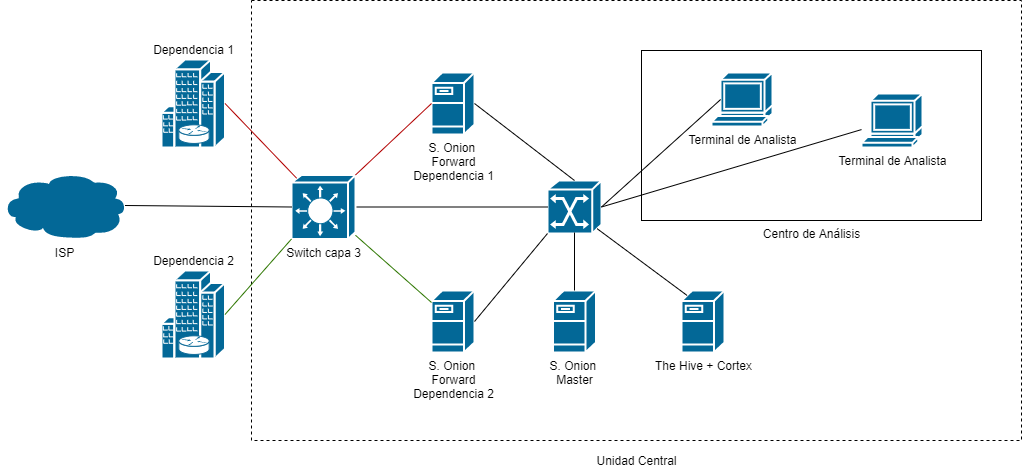
\includegraphics[width=1\textwidth]{./iteracion_1_imagenes/figura_33_arquitectura_despliegue_proyecto.png}
        \caption{Arquitectura de Despliegue}
        \label{fig:topologia_despliegue_proyecto}
    \end{figure}
    \FloatBarrier
    En la Figura \ref{fig:topologia_despliegue_proyecto} se muestra la topología de despliegue del proyecto. La figura 5.1 se muestra la topología de prueba donde se instalo Security Onion. En ella se observa el proveedor ISP de conexión a internet y por consiguiente al exterior de la organización, el switch de capa 3 al que están conectadas las dependencias cuyos enlaces fueron seleccionados para ser monitoreados para este proyecto, los nodos Forward de Security Onion y un switch de la red interna del CSIRT. Se observa que los enlaces “Dependencia 1 - switch capa 3” y el de “switch capa 3 - nodo Forward de Security Onion Dependencia 1” tienen el mismo color; esto se debe a motivos de representar el hecho de que el switch capa 3 fue configurado para reenviar el tráfico entre el enlace de este y la dependencia 1 hacia el nodo Forward mencionado. Una situación análoga ocurre entre la Dependencia 2 y el nodo Security Onion Forward Dependencia 2. \par
    El último eslabón de la conexión, el switch de capa 2, es el encargado de la red interna del CSIRT. A él se encuentran conectados las computadoras de los analistas y el nodo Master de Security Onion, los nodos Forward anteriormente mencionados y el servidor que aloja a TheHive y Cortex. Finalmente, los analistas pueden consultar y administrar los servidores correspondientes a los nodos Master y Forward de Security Onion así como al servidor que contiene a TheHive y Cortex. \par

   \end{section}
    
    \begin{section}{Selección de hardware} %cambiar el nombre de esta sección
        El primer paso consistió en examinar los requisitos de hardware mínimos y recomendados por cada uno de los fabricantes de los sistemas y subsistemas elegidos, al mismo tiempo que se analizaron, por un lado, las demandas de tráfico de red en el ambiente de prueba y por el otro los requerimientos sobre los datos y capacidades que se esperan obtener del proyecto. Se procedió a realizar un diagrama topológico en la infraestructura objetivo, con esta información y los datos anteriormente mencionados, se realizo una estimación del hardware necesario para el servidor central que albergó las correspondientes máquinas virtuales de este proyecto.\par
        Según el fabricante, los requerimientos de hardware para un entorno de producción con enlaces de 1 Gbps son son los que figuran en el Cuadro \ref{table:5}.
        
        \begin{table}[H]
        \centering
        \begin{tabular}{|m{9em}|m{9em}|m{9em}|m{9em}|}
        
            \hline 
                Requerimiento  & Nodo Master &  Nodo Forward & TheHive y Cortex \\ 
            \hline
                Cantidad de CPU - Arquitectura & Mínimo de 8 núcleos vCPU - x86-64 & Mínimo de 12 núcleos vCPU - x86-64 & Mínimo de 8 núcleos vCPU - x86-64 \\ 
            \hline
                Memoria RAM  & 12 a 128 GB & 128 a 256 GB & A partir de 8 GB \\ 
            \hline
                Almacenamiento necesario & Mínimo de 1 TB  & Mínimo de 540 GB & A partir de 60 GB \\
            \hline %linea final de tabla
        \end{tabular}
        \caption{Requerimientos de hardware recomendados por el fabricante para el monitoreo de un enlace de 1 Gbps}
        \label{table:5}
        \end{table}
        
        Debido a las restricciones en la disponibilidad del hardware, se realizó una implementación aproximada, teniendo en cuenta la optimización al máximo de los recursos disponibles. \par
	    Los nuevos requerimientos de hardware que se utilizaron se incluyen en el Cuadro \ref{table:12}.

        \begin{table}[H]
        \centering
        \begin{tabular}{|m{9em}|m{9em}|m{9em}|m{9em}|}
        
            \hline 
                Requerimiento  & Nodo Master &  Nodo Forward & TheHive y Cortex \\ 
            \hline
                Cantidad de CPU - Arquitectura & 8 nucleos vCPU - x86-64 & 10 nucleos vCPU - x86-64 & 8 nucleos vCPU - x86-64 \\ 
            \hline
                Memoria RAM  & A partir de 16 GB & A partir de 32 GB & A partir de 8 GB \\ 
            \hline
                Almacenamiento necesario & A partir de 500 GB  & A partir de 200 GB & A partir de 60 GB \\
            \hline %linea final de tabla
        \end{tabular}
        \caption{Requerimientos de hardware según el tipo de nodo desplegado. Los requerimientos varían según el tipo de enlace a monitorear.}
        \label{table:12}
        \end{table}
        \FloatBarrier
        %En este proyecto se monitorearon enlaces de 1 Gbps de ancho de banda, por lo tanto los requerimientos para el nodo forward se incrementaron a 10 núcleos vCPU y 32 GB de memoria RAM. \par
        En cuanto a los núcleos de CPU virtuales, su frecuencia era de 2.4 Ghz, basados en procesadores físicos Intel Xeon E5620. Las memorias RAM pertenecían a la tecnología DDR3 y su frecuencia de refresco de 2400 MHz.
        Los discos eran del tipo mecánico con una velocidad de transferencia para lectura de 196 MB/s y para escritura de 154 MB/s, con interfaz SATA III y 7200 rpm de velocidad de rotación. \par
    	Siguiendo el diagrama de la arquitectura de despliegue de la sección anterior, se optimizó al máximo el uso de los recursos del servidor disponible para permitir el despliegue de cuatro nodos: dos Forward y un Master de Security Onion, así como un cuarto conteniendo a TheHive y Cortex. \par

        \begin{subsection}{Configuración del entorno de virtualización}
        Para el entorno de virtualización se utilizó VMWare \cite{vmware}, concretamente la suite vSphere HyperVisor v6.7.0 u3. Este sistema operativo basado en Unix permite gestionar los recursos de hardware disponibles, almacenar imágenes de distintos sistemas operativos y crear máquinas virtuales con estos últimos. Durante el proceso de creación de una máquina virtual, se selecciona el sistema operativo deseado y es posible asignar distintas cantidades de memoria principal, secundaria, cantidad de vCPU, número y tipo de enlaces de red, entre otros parámetros. \par
         \begin{figure}[H]
          \centering
           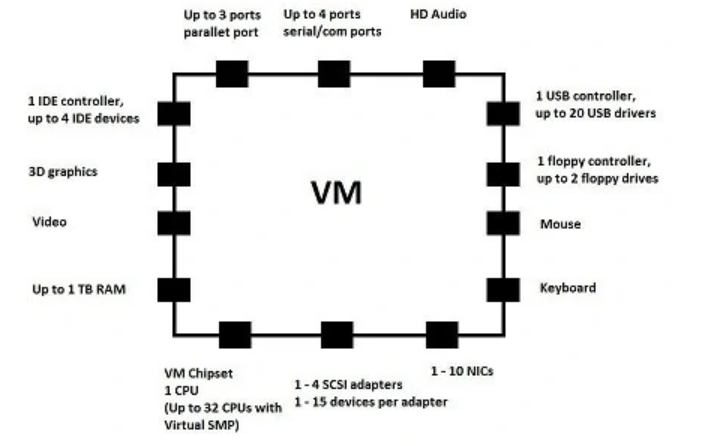
\includegraphics[width=0.7\textwidth]{./iteracion_2_imagenes/figura_34_diagrama_VM.png}
            \caption{ Diagrama de una máquina virtual desde el punto de vista de un HyperVisor\cite{vmware}}
            \label{fig:maquina_virtual}
        \end{figure}
        \end{subsection}
        
        \begin{subsection}{Definición y configuración de las redes a observar}
            Se decidió monitorear dos dependencias en base a un análisis del ancho de banda de las dependencias existentes, por lo tanto se seleccionaron las que mayor volumen de tráfico registraban en función de un registro histórico y mediciones propias realizadas a lo largo de una semana. Las dependencias seleccionadas tenían un enlace con ancho de banda de 1 Gbps cada una, con  velocidades promedio consideradas como la suma entre entrada y salida, entre 11,95 y 47,24 Mbps respectivamente; con picos poco frecuentes de 300 Mbps de tráfico, que no se contemplaron en los requisitos de hardware, por lo tanto habrá una posible pérdida de paquetes en estos casos. Se realizó un “port mirroring” de los puertos del switch capa 3 a los que están conectados estas dependencias y se los conecto con los respectivos enlaces de monitoreo de sendos nodos Forward de Security Onion. \par
            Los gráficos a continuación muestran el volumen del tráfico medido en dos periodos de tiempo distintos: Durante un día (exceptuando las horas en las que la actividad era mínima) y a lo largo de una semana. Si bien estos registros que se presentan a continuación corresponden a una sola de las dependencias, la restante tenía un comportamiento análogo. \par
            
            \begin{figure}[H]
                \centering
                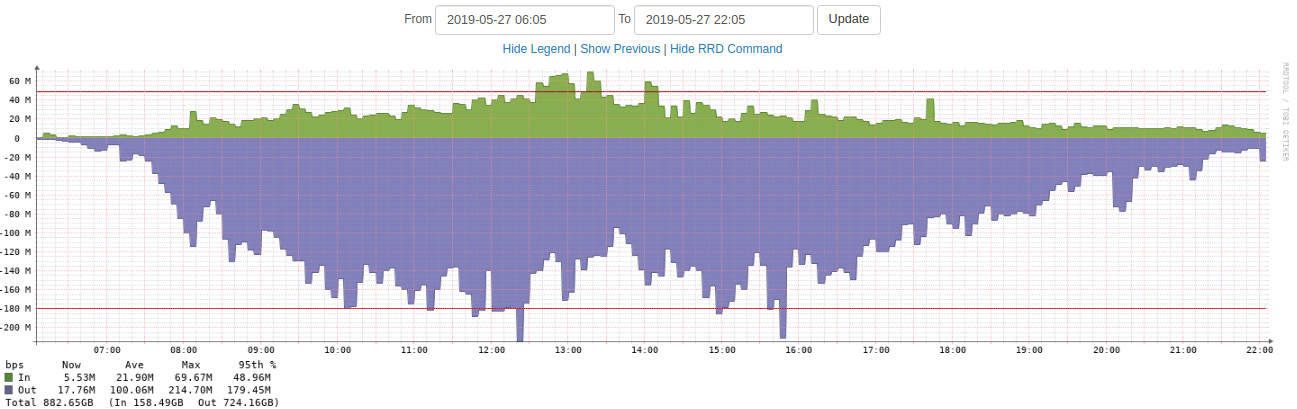
\includegraphics[width=0.7\textwidth]{./iteracion_2_imagenes/figura_35_trafico_dia.png}
                \caption{Tráfico correspondiente a una dependencia, medido durante un día, obviando las horas donde este es casi nulo}
                \label{fig:figura_35_trafico_dia}
            \end{figure}
            \begin{figure}[H]
            \centering
            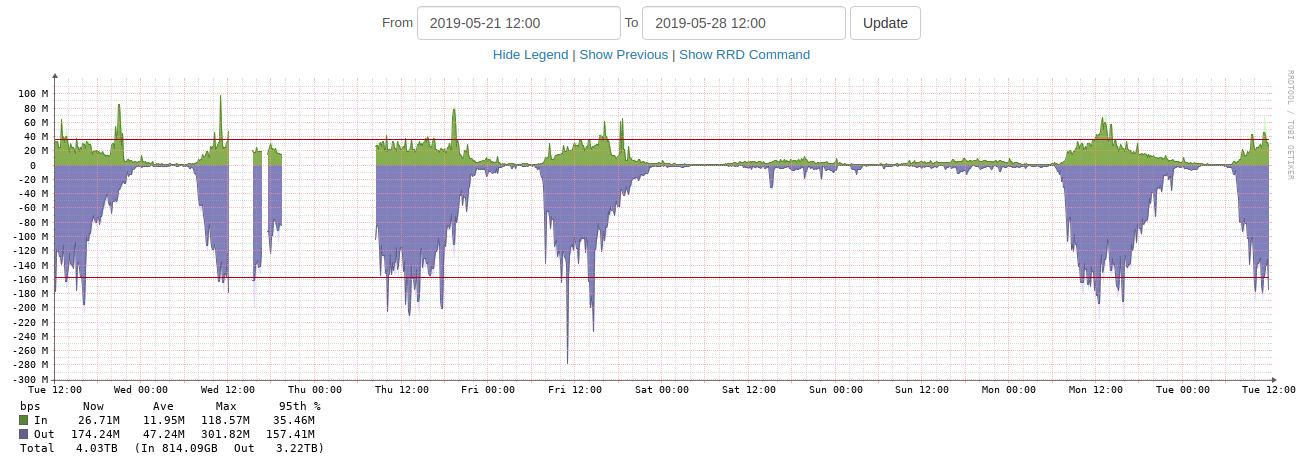
\includegraphics[width=0.7\textwidth]{./iteracion_2_imagenes/figura_36_trafico_semana.png}
            \caption{Tráfico medido durante el periodo correspondiente a una semana}
            \label{fig:figura_36_trafico_semana}
            \end{figure}
        \end{subsection}
    \end{section}
    
    \begin{section}{Configuración inicial del sistema base}
        Es posible instalar Security Onion en su versión 16.04 de dos maneras, sea mediante una ISO provista por los desarrolladores o bien mediante una serie de paquetes en una distribución Ubuntu \cite{ubuntu}. En este último caso será necesario contar con la distribución Ubuntu en su versión 16.04, ya que las distribuciones de Security Onion siguen a las distribuciones respectivas de Ubuntu; esto fue cierto hasta el año 2020 cuando se lanzaron nuevas versiones de Security Onion con soporte a otras distribuciones Linux: CentOS 7 y Ubuntu 18.04 y 20.04 aunque en el futuro se podrá desplegar en otros tipos de sistema Linux ya que desde la versión 2.x en adelante, el sistema se despliega en contenedores.

        \begin{subsection}{Instalación y configuración de Security Onion}
        Como se mencionó en la sección anterior, existen dos maneras de instalar Security Onion: a partir de una imagen ISO o mediante paquetes / contenedores. Se eligió para este proyecto la segunda opción, el despliegue mediante paquetes de la distribución 16.04 de Security Onion ya que al momento del desarrollo de este trabajo integrador era la versión estable del sistema. Por consiguiente, se dispuso de un sistema operativo Ubuntu Server 16.04 con la particularidad de tener dos discos montados: el principal para el sistema operativo y el secundario para los datos recolectados en un directorio /nsm: índices en el caso de un servidor Master y capturas de paquetes o logs en el caso de un nodo Forward. Luego de finalizada la instalación de Security Onion, es necesario elegir el rol (Master o Forward) del nodo mediante el asistente y posteriormente realizar la configuración del mismo. Para esto último, se cuenta con la guia del asistente integrado que permite elegir y configurar las interfaces disponibles (observación o administración); en el caso de un nodo Forward, elegir el motor IDS (Snort o Suricata). El último paso consiste en elegir entre dos tipos de modo de funcionamiento: Producción o Evaluación.
         \begin{figure}[H]
            \centering
            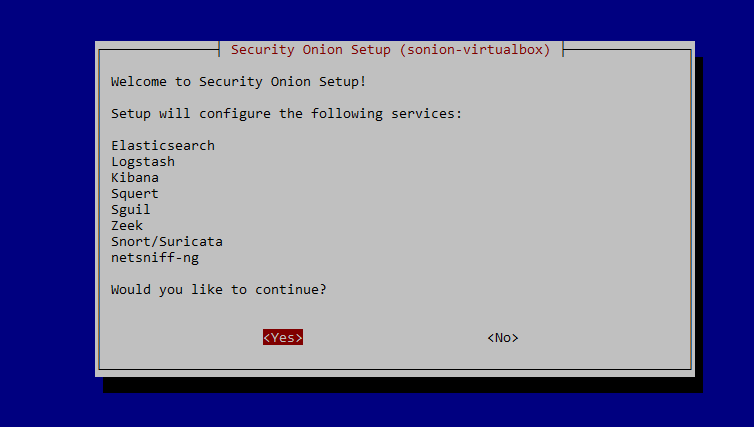
\includegraphics[width=0.7\textwidth]{./iteracion_2_imagenes/figura_37_sonion_conf.png}
            \caption{Asistente de instalación de Security Onion 16.04}
            \label{fig:figura_37_sonion_conf}
        \end{figure}
        \begin{figure}[H]
            \centering
            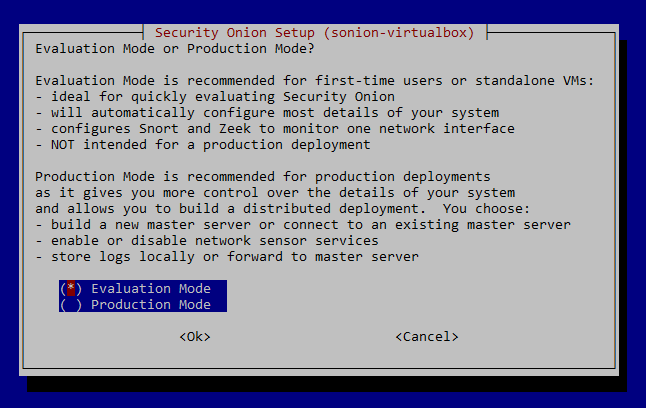
\includegraphics[width=0.7\textwidth]{./iteracion_2_imagenes/figura_38_sonion_modo.png}
            \caption{El asistente de instalación permite elegir el modo de despliegue}
            \label{fig:figura_38_sonion_modo}
        \end{figure}
        Con el objetivo de cumplir uno de los requerimientos no funcionales del proyecto, que implica la automatización del despliegue (instalación y configuración) del sistema, se utilizó una herramienta de administración automatizada de servidores llamada Ansible en su versión 2.8.4 para la cual se desarrollaron scripts YAML conteniendo la secuencia de instalación de los paquetes, configuraciones, rol del nodo (Forward o Master) y librerías requeridas para el apropiado funcionamiento del sistema
        \end{subsection}
        \begin{subsection}{Instalación y configuración de TheHive - Cortex}
        Para la instalación del gestor de incidentes, que tiene como componentes a  TheHive y Cortex, se utilizó  el sistema operativo Debian 10. En primer lugar se instaló TheHive, para ello fue necesario realizar la instalación previa de los componentes necesarios como las librerías de Java, Python y Elasticsearch; este último requirió una configuración en su archivo elasticsearch.yaml:
        
        \begin{figure}[H]
            \centering
            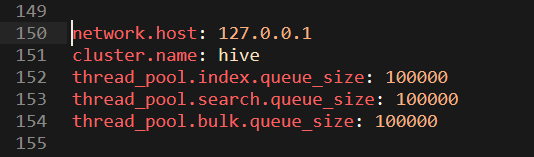
\includegraphics[width=0.7\textwidth]{./iteracion_2_imagenes/figura_39_thehive_conf_elastic.png}
            \caption{Configuración añadida a elasticsearch.yaml para la instalación de TheHive}
            \label{fig:figura_39_thehive_conf}
        \end{figure}
        Finalmente, los últimos pasos para la instalación de TheHive consisten en habilitar e iniciar el servicio de elasticsearch, agregar el repositorio que contiene los paquetes de TheHive, instalarlo y luego habilitar el servicio para poder iniciarlo. \par
        En cuanto a Cortex, el proceso es similar al anteriormente descrito para TheHive, donde una vez descargados e instalados los paquetes de Cortex con su correspondiente secuencia de habilitación e inicio; se procedió a descargar del repositorio los responders y analyzers respectivos. Por último, se modifica el archivo de configuración de Cortex para indicar la ubicación del directorio que contiene los responders y analyzers mencionados anteriormente. \par
        Posteriormente se actualizó la base de datos elasticsearch mediante la GUI web de Cortex, se creó un superusuario y luego las organizaciones donde se administrarán usuarios comunes y analyzers; es necesario crear un usuario con el rol de administrador de organizaciones. Las organizaciones tendrán habilitados y configurados determinados responders y analyzers según sea necesario. \par
        El último paso del proceso consiste en comunicar TheHive y Cortex entre sí. Para ello se genera una API key en Cortex que será usada como parte de las modificaciones necesarias al archivo application.conf de TheHive. Las modificaciones completas que se realizaron al mencionado archivo se pueden apreciar en la Figura \ref{fig:figura_40_thehive_cortex_conf}:\par
        
        \begin{figure}[H]
            \centering
            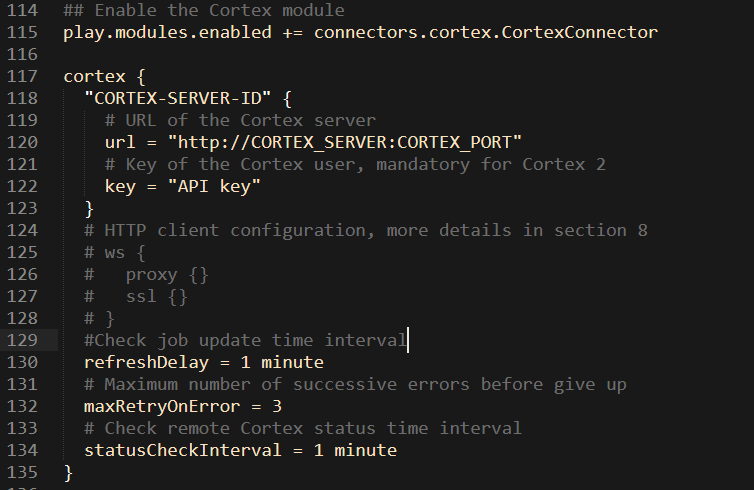
\includegraphics[width=0.7\textwidth]{./iteracion_2_imagenes/figura_40_thehive_cortex_conf.png}
            \caption{Modificación al archivo application.conf de TheHive para la comunicación con Cortex}
            \label{fig:figura_40_thehive_cortex_conf}
        \end{figure}
        \end{subsection}
        
    \end{section}
   
   %\begin{section}{Configuración de acciones automáticas}
%        El mecanismo elegido para automatizar las acciones fue mediante webhooks, para ello fue necesario implementar un entorno de virtualización en el mismo servidor donde se encuentran alojados TheHive y Cortex. Para ello se optó por utilizar el módulo de python “venv”, lo que requirió la instalación de Python 3.6 como primer paso. En segundo lugar se modificó el archivo application.conf de TheHive que se mencionó en la sección anterior para permitir la comunicación con el puerto  del entorno de virtualización. En tercer lugar se verificó que en el nodo Master de Security Onion las reglas de ElastAlert tengan los campos necesarios configurados como observables ya que estos serán necesarios posteriormente dado que en TheHive están creados los observables que esperan esta información (source\_ip, destination\_ip, source\_port, destination\_port, alert, classification, category, etc). \par
%        Satisfechos los pasos anteriores, la instalación siguió los siguientes pasos:
%        \begin{itemize}
 %           \item Se creo una carpeta con el nombre webhooksenv
 %           \item Un entorno virtual fue creado y activado en la mencionada carpeta
 %           \item Se procedió a instalar las librerias necesarias: Flask, Gunicorn, Wheel, Request y Netaddr.
 %           \item Se desactivo el entorno virtual y se habilitó en el firewall el puerto 5000.
%            \item Se agregaron y modificaron valores al archivo de parámetros que utiliza webhooks.
%            \item Se inició y comprobó el estado del servicio.
%        \end{itemize}
%        Finalmente, se modificaron los archivos de configuración de TheHive y Cortex para actualizar la información necesaria referida a los webhooks.

   %\end{section}